% \documentclass[conference]{IEEEtran}
\documentclass[a4paper,11pt]{article}
\usepackage[a4paper, total={6.6in, 9.8in}]{geometry}
\usepackage{graphicx}
\graphicspath{ {./images/output/} }
\usepackage{caption}
\usepackage[english]{babel}
\usepackage{titling}
\usepackage{float}
\usepackage{amsmath}
\usepackage{minted}
\usepackage{minted}
\usepackage{multicol}
\usepackage{array}
\usepackage{setspace}
\usepackage{placeins}
\usepackage{parskip}

\title{Experiment 4\\ Observation of Various Features of an EEG Signal Collected from Kaggle MNE Dataset}
\author{}
\date{}

\begin{document}
\vspace*{\fill}
\begin{center}

    \emph{Heaven's Light is Our Guide} \\
    \textbf{Rajshahi University of Engineering and Technology} \\

    \begin{figure}[H]
        \centering
        
\includegraphics[scale=.34]{images/RUET_logo.png}
        \label{fig:ruet_logo}
    \end{figure}
    \vspace{5mm}

    \textbf{Course Code}\\
    ECE 4144\\
    \vspace{3mm}
    \textbf{Course Title}\\
    Biomedical Engineering Sessional

    \vspace{5mm}
    \textbf{Experiment Date:} {August 06, 2025},\\
    \textbf{Submission Date:} {August 13, 2025}\\

    \vspace{5mm}
    \textbf{Lab Report 3: \\
        Experimental Observation of Various Features of an ECG
        Signal Collected from PhysioNet Public Dataset}

    \vspace{15mm}

    \begin{tabular}{c|c}
        \textbf{Submitted to} & \textbf{Submitted by} \\
        Md Mayenul Islam      & Md. Tajim An Noor     \\
        Assistant Professor   & Roll: 2010025         \\
        Dept of EEE, Ruet     &                       \\
    \end{tabular}

\end{center}
\vspace*{\fill}

\newpage

\maketitle
\pagenumbering{gobble}

\vspace{-5em}

\section*{Objectives}
\begin{itemize}
    \item To analyze and observe key features of EEG signals from the Kaggle MNE database.
    \item To identify and visualize major EEG frequency bands.
\end{itemize}

\section*{Theory}
Electroencephalography (EEG) is a non-invasive method for recording brain electrical activity via scalp electrodes, capturing summed neuronal post-synaptic potentials. EEG signals are categorized into frequency bands—delta (0.5–4 Hz), theta (4–8 Hz), alpha (8–13 Hz), beta (13–30 Hz), and gamma (30–100 Hz)—each linked to specific brain states such as sleep, relaxation, or alertness~\cite{niedermeyer2005electroencephalography}. While EEG offers high temporal resolution for studying dynamic brain activity, signals often require preprocessing to remove artifacts. This experiment analyzes Kaggle MNE EEG data~\cite{kagglemnedataset} to observe and interpret these characteristic frequency features.

\section*{Dataset Description}
The Kaggle MNE EEG Dataset provides multi-channel EEG recordings from healthy subjects. Each recording includes 64 scalp channels (10-20 system), sampled at 160 Hz, with metadata on channels and subjects. The dataset is widely used for EEG analysis and frequency band studies~\cite{kagglemnedataset}.

\textbf{Key details:}
\begin{itemize}
    \item \textbf{Source:} Kaggle MNE EEG Dataset~\cite{kagglemnedataset}
    \item \textbf{Channels:} 64 (10-20 system)
    \item \textbf{Sampling Rate:} 160 Hz
    \item \textbf{Format:} Multichannel time-series
\end{itemize}

\section*{Tools Used}
\begin{itemize}
    \item \textbf{Jupyter Notebook}
    \item \textbf{VS Code}
    \item \textbf{\LaTeX}
\end{itemize}

\section*{Output}
\begin{figure}[H]
    \centering
    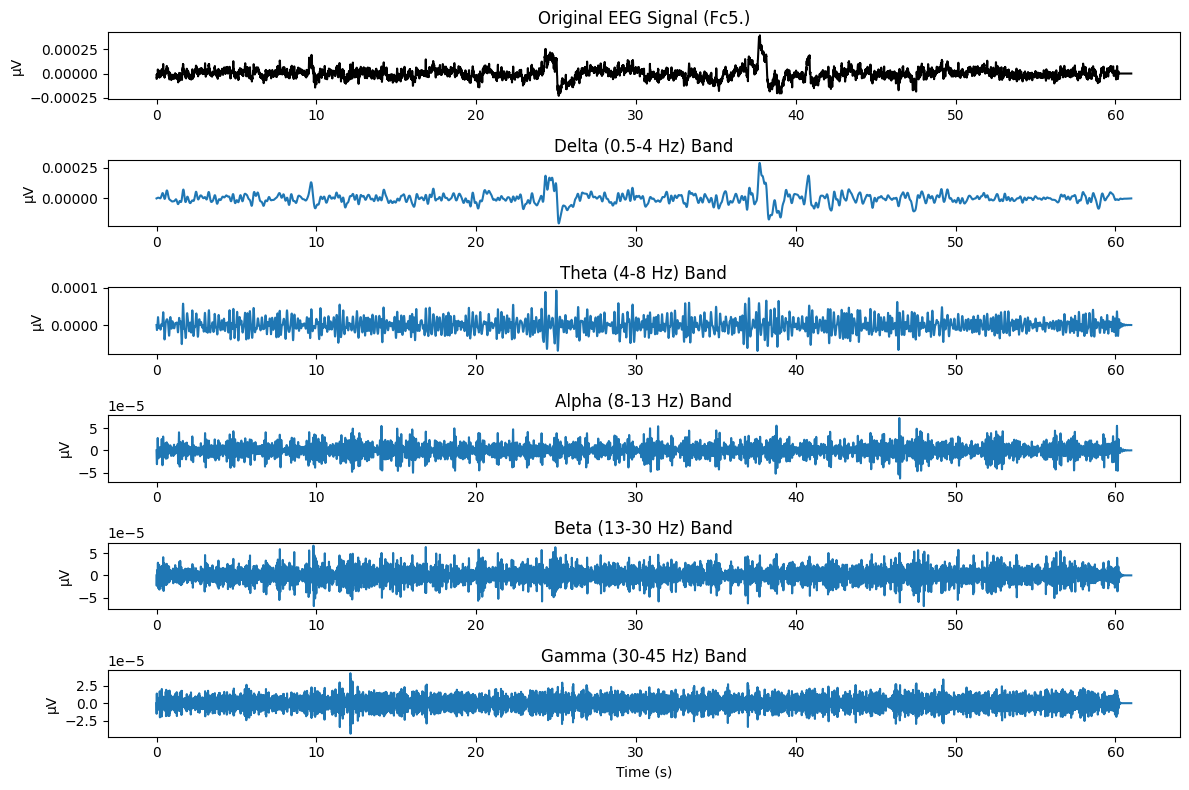
\includegraphics[width=0.68\textwidth]{output.png}
    \caption{Observation of EEG signals}
    \label{fig:raw_eeg}
\end{figure}

\vspace{-1em}

\begin{minted}{console}
EEG Band Statistical Features:
                  Mean  Std Dev  Variance  Skewness  Kurtosis  RMS  Band Power
Delta (0.5-4 Hz)   0.0      0.0       0.0    0.6923    6.4781  0.0         0.0
Theta (4-8 Hz)    -0.0      0.0       0.0    0.2412    0.8139  0.0         0.0
Alpha (8-13 Hz)   -0.0      0.0       0.0    0.0061    0.7088  0.0         0.0
Beta (13-30 Hz)   -0.0      0.0       0.0    0.0018    0.9454  0.0         0.0
Gamma (30-45 Hz)  -0.0      0.0       0.0   -0.0029    0.3404  0.0         0.0
\end{minted}

% \vspace{-1em}

\section*{Analysis}
The outputs include the original EEG signal and band-specific signals (Delta, Theta, Alpha, Beta, Gamma) obtained via bandpass filters. For each band, statistical features—mean, standard deviation, variance, skewness, kurtosis, RMS, and band power—were computed. These results highlight how different brain rhythms appear in EEG and demonstrate the effectiveness of signal processing for isolating and analyzing specific components.

% \vspace{-1em}

\section*{Discussion \& Conclusion}
The experiment demonstrated key EEG features using the Kaggle MNE dataset. Raw EEG signals showed characteristic brainwave patterns, and bandpass filtering isolated the delta, theta, alpha, beta, and gamma bands. Statistical analysis confirmed the separation of these frequency bands. The results highlight the importance of preprocessing and spectral analysis for extracting meaningful information from EEG data.

\bibliographystyle{IEEEtran}
\renewcommand{\bibname}{References}
\bibliography{ref}

\end{document}
